%% scatterplots.tex
%% Author: Leighton Pritchard
%% Copyright: James Hutton Institute
%% Inferences of correlation from scatterplots are sensitive to presentation

% Frame template 
\begin{frame}
  \frametitle{Scatterplots
  \footnote{\tiny{\href{http://www.datavizcatalogue.com/}{http://www.datavizcatalogue.com/}}}
  }
  \begin{alertblock}{Scatterplots should be awesome:}
    \begin{itemize}
      \item Positions on common scale (lowest error representation)
      \item Show all data: outliers, sample sizes, trends, etc.
    \end{itemize}
  \end{alertblock}
  \begin{center}
    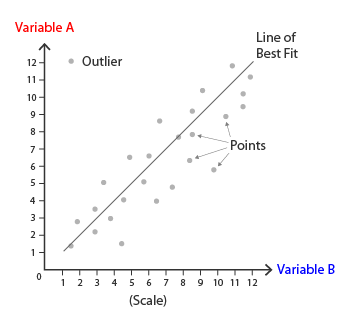
\includegraphics[width=0.5\textwidth,valign=t]{images/scatterplot1}
    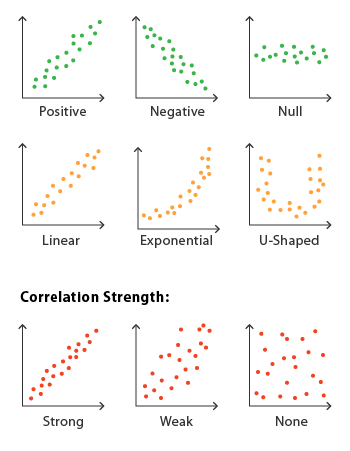
\includegraphics[width=0.33\textwidth,valign=t]{images/scatterplot2}
  \end{center}
\end{frame}

% Frame template 
\begin{frame}
  \frametitle{Framing affects interpretation
  \footnote{\tiny{\href{http://dx.doi.org/10.1126/science.216.4550.1138}{Cleveland \textit{et al.} (1982) \textit{Science} doi:10.1126/science.216.4550.1138}}}
  }
  \textcolor{hutton_green}{Point cloud size affects interpretation of correlation} \\
  \textcolor{hutton_blue}{(more diffuse interpreted as lower correlation coefficient)}
  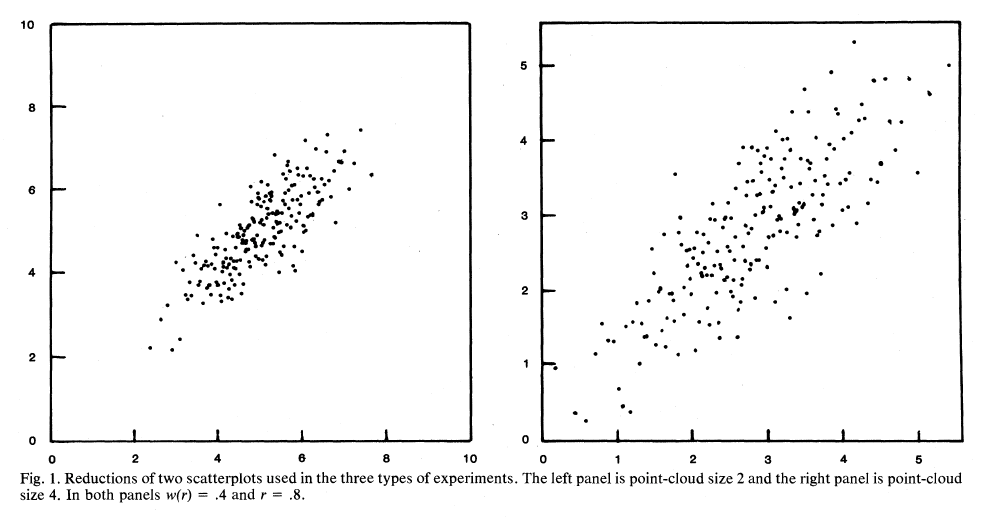
\includegraphics[width=1\textwidth]{images/scatterplot_framing}    
\end{frame}

% Frame template 
\begin{frame}
  \frametitle{Interpreting correlation is difficult
  \footnote{\tiny{\href{http://dx.doi.org/10.7717/peerj.589}{Fisher \textit{et al.} (2014) \textit{PeerJ} doi:10.7717/peerj.589}}}
  }
  \begin{alertblock}{People don't judge significance well}
    \begin{itemize}
      \item 47.4\% of significant relationships correctly classified
      \item 74.6\% of non-significant relationships correctly classified
    \end{itemize}
  \end{alertblock}
  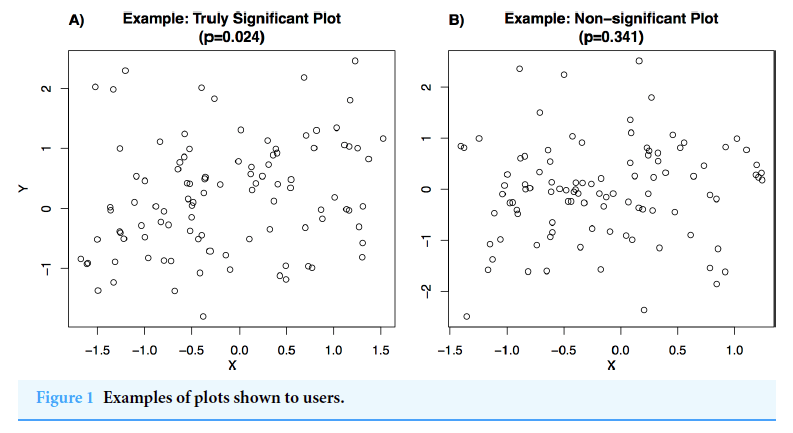
\includegraphics[width=0.5\textwidth]{images/scatterplot_fisher1}    
  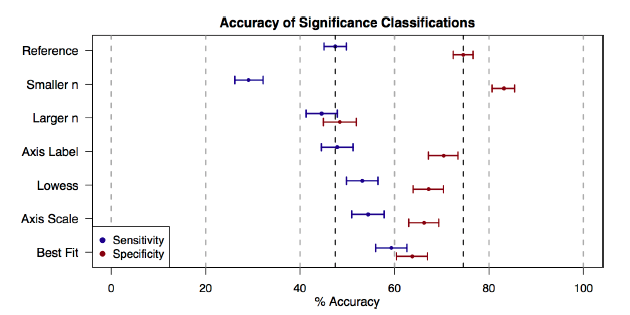
\includegraphics[width=0.5\textwidth]{images/scatterplot_fisher2}    
\end{frame}